\chapter{Θεωρητικό υπόβαθρο}

%Το \en{Lorem Ipsum} είναι απλά ένα κείμενο χωρίς νόημα για τους επαγγελματίες της τυπογραφίας και στοιχειοθεσίας \cite{LoremIpsumAll}. Το \en{Lorem Ipsum} είναι το επαγγελματικό πρότυπο όσον αφορά το κείμενο χωρίς νόημα, από τον 15ο αιώνα, όταν ένας ανώνυμος τυπογράφος πήρε ένα δοκίμιο και ανακάτεψε τις λέξεις για να δημιουργήσει ένα δείγμα βιβλίου. Όχι μόνο επιβίωσε πέντε αιώνες, αλλά κυριάρχησε στην ηλεκτρονική στοιχειοθεσία, παραμένοντας με κάθε τρόπο αναλλοίωτο. Έγινε δημοφιλές τη δεκαετία του '60 με την έκδοση των δειγμάτων της \en{Letraset} όπου περιελάμβαναν αποσπάσματα του \en{Lorem Ipsum}, και πιο πρόσφατα με το λογισμικό ηλεκτρονικής σελιδοποίησης όπως το \en{Aldus PageMaker} που περιείχαν εκδοχές του \en{Lorem Ipsum}.
\section{\en{Web Framework} και Βασικές Τεχνολογίες Ανάπτυξης}

\subsection{\en{Django Framework}}

Το \en{Django} είναι ένα \en{backend framework} το οποίο βασίζεται στη γλώσσα προγραμματισμού \en{Python}. 
Το \en{Django} βοηθάει στο να στηθεί γρήγορα μία εφαρμογή ανάπτυξης ιστού έτσι ώστε να μπορούμε να εστιάσουμε στη σύνταξη της εφαρμογής και της λειτουργικότητάς της χωρίς να χρειάζεται να ανακαλύψουμε ξανά τον τροχό.
Είναι δωρεάν και ανοιχτού κώδικα. Ορισμένες από τις πιο μεγάλες εταιρίες στον πλανήτη χρησιμοποιούν την ικανότητα του
να κλιμακώνεται γρήγορα και με ευελιξία για να ανταποκρίνεται στις μεγαλύτερες απαιτήσεις κίνησης. Στη δικιά μας περίπτωση χρησιμοποιήθηκε το συγκεκριμένου
\en{Framework} γιατί θα μας έδινε τη δυνατότητα να φτιάξουμε μία εφαρμογή με μεγάλη επεκτασιμότητα και παράλληλα να μπορέσουμε να ενσωματώσουμε μέσα διαφορετικές τεχνολογίες.

Παράλληλα με το \en{Django} χρησιμοποιήθηκαν έτοιμες βιβλιοθήκες της \en{Python} προκειμένου να μπορέσουν να εκτελεστούν βασικές λειτουργίες της εφαρμογής όπως 
τα πρωτοκολλα επικοινωνίας. Στην ενότητα 4.3 παρουσιάζονται οι βιβλιοθήκες που χρησιµοποιήθηκαν και κάποια βασικά χαρακτηριστικά τους.

\subsection{Διαχείρηση εκδόσεων (\en{Version Control}) με \en{Git} και \en{GitHub} }

Το \en{Git} είναι ένα σύγχρονο σύστημα ελέγχου εκδόσεων (γνωστό και ως σύστημα διαχείρισης αναθεωρήσεων ή πηγαίου κώδικα), 
σχεδιασμένο με έμφαση στην ταχύτητα, την ακεραιότητα των δεδομένων και την υποστήριξη κατανεμημένων, μη γραμμικών ροών εργασίας. 
Στην παρούσα διπλωματική εργασία, θα αξιοποιήσουμε το \en{Git} για να διασφαλίσουμε την ορθή διαχείριση των εκδόσεων του λογισμικού, 
τόσο κατά τη διάρκεια της ανάπτυξης όσο και για την πιθανή μελλοντική χρήση και εξέλιξη της δουλειάς μας. Το \en{GIT} συνεπώς είναι απαραίτητο σε κάθε σοβαρό 
έργο ανάπτυξης, και αυτό δεν αποτελεί εξαίρεση. Παρέχει γρήγορη ανάπτυξη κώδικα, έκδοση και επιτρέπει διακλαδώσεις. Έχοντας το εγκατεστημένο τόσο στον τοπικό υπολογιστή ανάπτυξης όσο και στο περιβάλλον παραγωγής, διευκολύνει και επιταχύνει τη διαδικασία ανάπτυξης στο παραγωγικό περιβάλλον.
Τον ήδη δοκιμασμένο κώδικα στο τοπικό περιβάλλον ανάπτυξης. Η έκδοση παρέχει τη δυνατότητα επαναφοράς σε προηγούμενες εκδόσεις κώδικα σε
περίπτωση  κάποιο άγνωστο σφάλμα εμφανιστεί σε μια νεότερη έκδοση. 

\section{Αυτοματοποίηση Δικτύων και Διασύνδεση με Δικτυακές Συσκευές}

\subsection{Αυτοματοποίηση Διαχείρησης Δικτύου}

Η αυτοματοποίηση δικτύου δεν περιορίζεται μόνο στη διαμόρφωση συσκευών. 
Αντιθέτως, το πιο σημαντικό μέρος της αυτοματοποίησης δικτύου, που συμβάλλει στη μείωση των ανθρώπινων σφαλμάτων, 
είναι η δυνατότητα που παρέχει στους διαχειριστές να αυτοματοποιούν διαδικασίες για τη διενέργεια ελέγχων συμμόρφωσης και 
επικύρωσης της τρέχουσας διαμόρφωσης ή οποιασδήποτε διαμόρφωσης πρόκειται να εφαρμοστεί.

Αυτό έχει ως αποτέλεσμα τη μείωση του χρόνου υλοποίησης των αλλαγών στο δίκτυο και του κινδύνου διακοπής ή διατάραξης της υπηρεσίας, 
ενώ ελαχιστοποιεί την πιθανότητα ανθρώπινου λάθους και διασφαλίζει την ευθυγράμμιση με τις πολιτικές του δικτύου.Μία ακόμη διαδικασία που μπορεί να 
αυτοματοποιηθεί είναι η επίλυση προβλημάτων. Όταν προκύπτει κάποιο πρόβλημα στο δίκτυο, το πρώτο βήμα για την αντιμετώπισή του είναι η συλλογή πληροφοριών. 
Η συλλογή πληροφοριών από κάθε συσκευή μπορεί να είναι χρονοβόρα και περίπλοκη, κάτι που είναι κρίσιμο, διότι συνήθως, στο μεταξύ, το δίκτυο ή ένα μέρος του παραμένει 
εκτός λειτουργίας.

Με τη χρήση της αυτοματοποίησης δικτύου, μπορούμε να αυτοματοποιήσουμε τις εντολές που απαιτούνται για τη 
συλλογή των απαραίτητων πληροφοριών για την επίλυση προβλημάτων και να έχουμε πρόσβαση σε αυτές σε πραγματικό χρόνο.
Η προγραμματική συλλογή αυτών των πληροφοριών επιτρέπει και τον έλεγχο τους σε πραγματικό χρόνο. 

Η παρούσα διπλωματική εργασία βασίστηκε σε μια συναφή μελέτη (\selectlanguage{english} \url{https://github.com/dmfigol/network-programmability-stream} \selectlanguage{greek}), η οποία υλοποιήθηκε από έναν μηχανικό που ανέπτυξε μια παρόμοια εφαρμογή χρησιμοποιώντας το \en{Django}. Στην εργασία του, ο δημιουργός εστίασε στην υλοποίηση βασικών λειτουργιών, αξιοποιώντας ένα διαφορετικό περιβάλλον, καθώς είχε πρόσβαση σε εικονικές συσκευές. Συνεπώς, δεν απαιτήθηκε η χρήση του \en{GNS3} για δοκιμές.

Οι κύριες λειτουργίες που ανέπτυξε περιλάμβαναν την καταγραφή των συσκευών και τη διαμόρφωση διευθύνσεων \en{IP}. Αξίζει να σημειωθεί ότι, λόγω της επαγγελματικής μου εμπειρίας στην \en{Ericsson}, έχω έρθει σε επαφή με πιο προηγμένα συστήματα αυτού του τύπου, όπως το \en{ENM (Ericsson Network Manager)}[24]. Το συγκεκριμένο σύστημα παρέχει εξειδικευμένες λύσεις για τη διαχείριση εξαιρετικά πολύπλοκων τηλεπικοινωνιακών υποδομών, όπου η διαχείριση, η παραμετροποίηση και η παρακολούθηση των δικτυακών συσκευών είναι κρίσιμης σημασίας

Ο έλεγχος πληροφοριών σε πραγματικό χρόνο και η άμεση λήψη αποφάσεων, όταν μεταβάλλεται μια κρίσιμη παράμετρος, όπως το \en{MTU}, αποτελεί μία σημαντική πτυχή της αυτοματοποιημένης διαχείρισης δικτύων, γνωστή ως αυτοματοποιημένη παρακολούθηση.
Το \en{MTU} (\en{Maximum Transmission Unit}) καθορίζει το μέγιστο μέγεθος των δεδομένων που μπορούν να μεταφερθούν σε ένα πακέτο μέσω ενός συγκεκριμένου δικτυακού μέσου. Η συνεχής παρακολούθηση τέτοιων παραμέτρων μπορεί να συμβάλει στην έγκαιρη ανίχνευση πιθανών προβλημάτων, όπως η δυσλειτουργία ενός δικτυακού \en{interface}.
Ακόμη περισσότερο, η αυτοματοποιημένη παρακολούθηση παίζει καθοριστικό ρόλο στην πρόληψη βλαβών που προκύπτουν από αποτυχίες υλικού, επιτρέποντας την έγκαιρη διάγνωση και την ελαχιστοποίηση του χρόνου διακοπής λειτουργίας του δικτύου. Στην παρούσα διπλωματική εργασία δεν υλοποιήθηκε αυτοματοποιημένη παρακολούθηση αλλά αυτοματοποιημένη συλλογή πληροφοριών.


\section{Βιβλιοθήκες της \en{Python} για \en{Network automation}}

\subsection{\en{Paramiko}}
Το \en{Paramiko} είναι μια βιβλιοθήκη της \en{Python} που υλοποιεί το πρωτόκολλο \en{SSH} έκδοσης 2 σε \en{Python}, παρέχοντας λειτουργικότητα τόσο πελάτη όσο και διακομιστή.
Η \en{Paramiko} βασίζεται στην κρυπτογραφία για τη λειτουργία κρυπτογράφησης, η οποία χρησιμοποιεί επεκτάσεις \en{C} και \en{Rust}.
Οποιαδήποτε συσκευή που μπορεί να ρυθμιστεί μέσω \en{SSH} μπορεί επίσης να ρυθμιστεί από την \en{Python} με σενάρια με τη χρήση αυτής της μονάδας.

\subsection{\en{Netmiko}}
Το \en{Netmiko} είναι µια βιβλιοθήκη \en{Python} ανοικτού κώδικα η οποία μπορεί να υποστηρίξει πολλές 
διαφορετικές συσκεύες διαφορετικών προµηθευτών(\en{Cisco},\en{Juniper},\en{Arista} και άλλοι) που σηµαίνει ότι πολλές συσκευές µπορούν 
να ρυθµιστούν από την \en{python} χρησιµοποιώντας το \en{Netmiko}. 
Το \en{framework} αυτό χρησιμοποιήθηκε στην εργασία γιατί απλοποιεί τη σύνδεση με συσκευές μέσω \en{SSH}, αφαιρώντας την πολυπλοκότητα στη διαχείριση διαφορετικών πρωτοκόλλων και 
τύπων συσκευών.


Το \en{Netmiko} περιλαμβάνει επίσης ενσωματωμένες λειτουργίες για την εκτέλεση εντολών και τη διαχείριση ρυθμίσεων, επιταχύνοντας την ανάπτυξη λύσεων.
Υποστηρίζει ασύγχρονες λειτουργίες για αποτελεσματική διαχείριση πολλαπλών ταυτόχρονων συνδέσεων, κάτι που είναι κρίσιμο για μεγάλης κλίμακας δίκτυα. Επιπλέον, έχει ισχυρή 
κοινότητα και τακτικές ενημερώσεις, διευκολύνοντας την υποστήριξη και την επίλυση προβλημάτων.
Τόσο το \en{Paramiko} όσο και το \en{Netmiko} αποτελούν εναλλακτικές επιλογές για συσκευές που δεν υποστηρίζουν \en{APIs} επειδή βασίζεται στο \en{SSH} πρωτόκολλο.


\subsection{\en{Napalm}}
Το \en{NAPALM} (\en{Network Automation and Programmability Abstraction Layer with Multivendor support}) είναι μια βιβλιοθήκη \en{Python} που υλοποιεί ένα σύνολο λειτουργιών για την αλληλεπίδραση με διαφορετικά λειτουργικά συστήματα συσκευών δικτύου χρησιμοποιώντας ένα ενοποιημένο \en{API}.
Το \en{NAPALM} υποστηρίζει διάφορες μεθόδους σύνδεσης με τις συσκευές, χειρισμού των ρυθμίσεων ή ανάκτησης δεδομένων. Το \en{Napalm} συνεπώς είναι μια βιβλιοθήκη \en{Python} που παρέχει ένα \en{API}
\en{(Application Programming Interface)} για την εργασία με συσκευές δικτύου. Έχει σχεδιαστεί για να απλοποιεί την
αυτοματοποίηση και τη διαχείριση του δικτύου με την αφαίρεση των υποκείμενων λεπτομερειών που σχετίζονται με τον εκάστοτε προμηθευτή και την παροχή μιας συνεπούς διεπαφής σε διαφορετικά δίκτυα. 
συσκευών.


Το \en{Napalm} επιτρέπει στους μηχανικούς και τους διαχειριστές δικτύων να αυτοματοποιούν κοινές εργασίες διαχείρισης δικτύου, όπως η διαμόρφωση, η παροχή, η παρακολούθηση και η 
αντιμετώπιση προβλημάτων. Υποστηρίζει πολλούς προμηθευτές συσκευών δικτύου, συμπεριλαμβανομένων των \en{Cisco}, \en{Juniper}, \en{Arista} και \en{Huawei}.
Το \en{Napalm} παρέχει ένα σύνολο κοινών λειτουργιών που μπορούν να εκτελεστούν σε συσκευές δικτύου, όπως η ανάκτηση πληροφοριών διαμόρφωσης, η εφαρμογή διαμόρφωσης 
αλλαγών, έλεγχος στατιστικών στοιχείων διασύνδεσης και συλλογή πληροφοριών τοπολογίας δικτύου παρέχει επίσης χαρακτηριστικά όπως υποστήριξη επαναφοράς, επικύρωση διαμόρφωσης 
αλλαγών διαμόρφωσης, και σύγκριση των διαφορών διαμόρφωσης μεταξύ συσκευών.


Το \en{Napalm} μπορεί να συνδυαστεί με βιβλιοθήκες \en{Python} όπως οι \en{Netmiko}, \en{Paramiko} και \en{Ansible} για τη δημιουργία σύνθετων ροών εργασίας αυτοματισμού δικτύου. Μπορεί επίσης να ενσωματωθεί με δημοφιλή εργαλεία παρακολούθησης δικτύου, όπως το \en{Prometheus} και το \en{Grafana}, για την παρακολούθηση της απόδοσης του δικτύου σε πραγματικό χρόνο. Η συνάρτηση \en{get network driver} της βιβλιοθήκης \en{NAPALM} χρησιμοποιείται στην εφαρμογή μας  προκειμένου το  \en{User Interface} του \en{Django}  να αποκτήσει έναν οδηγό δικτύου που επιτρέπει την αλληλεπίδραση με τις συσκευές της \en{Cisco} μέσω ενός ενιαίου \en{API}. Αυτό διευκολύνει την αυτοματοποίηση και τη διαχείριση των συσκευών χρησιμοποιώντας το πρωτόκολλο \en{SSH}.


\subsection{\en{Cisco IOS} και \en{REST APIs} για Δικτυακές Συσκευές της \en{Cisco}  }

Το \en{IOU} (\en{Cisco IOS on UNIX}) είναι µια εικονική έκδοση του λογισµικού \en{IOS} της \en{Cisco} που µπορεί να χρησιµοποιηθεί για σκοπούς προσοµοίωσης και δοκιµής δικτύου. Επιτρέπει στους µηχανικούς δικτύου να δηµιουργούν εικονικές τοπολογίες δικτύου και να εξασκούνται σε διάφορες εργασίες δικτύου, όπως η διαµόρφωση δροµολογητών και µεταγωγέων, χωρίς να απαιτείται φυσικό υλικό. 


Το \en{IOS} μπορεί να τρέχει κατευθείαν πάνω σε υλικό, δηλαδή μπορεί να εγκατασταθεί απευθείας πάνω στα \en{router} και στα \en{switches} . Το \en{IOU} είναι λογισμικό το οποίο μπορεί να τρέξει το λογισμικό (\en{IOS}) ακόμα και σε \en{PC} προσομοιώνοντας με αυτόν τον τρόπο λογισμικό δικτυακών συσκευών χωρίς την ανάγκη ύπαρξης συγκεκριμένου υλικού. Στην εφαρμογή μας χρησιμοποιήθηκαν τέτοιες εικονικές εκδόσεις προκειμένου να προσομειώσουμε τις \en{Cisco} συσκευές καθώς δεν υπήρχε διαθέσιμο πειραματικό υλικό τέτοιο που να μας επιτρέψει την προσομείωση IOS. Τα \en{CISCO IOU} είναι εύκολα στην εγκατάσταση και την προσωμείωσή τους συνεπώς κάνουν και τη δημιουργία του \en{testbed} ευκολότερη.

Στο πλαίσιο της δημιουργίας της εφαρμογής αξιοποιήθηκε και το \en{REST} πρωτόκολλο. Ο λόγος που το χαρακτηρίζω ως \en{REST} είναι επειδή η διαδικασία αυτή βασίζεται στη θεμελιώδη αρχή του \en{HTTP} \en{request-response} μοντέλου: όταν ένας χρήστης εισάγει ένα \en{URL} στον \en{browser}, πραγματοποιείται ένα \en{HTTP request} προς τον \en{server}, ο οποίος στη συνέχεια επιστρέφει την κατάλληλη απάντηση, στην προκειμένη περίπτωση το κάθε αρχείο \en{html} που υλοποιήσαμε μέσα από το \en{views.py} επιστρέφει ως \en{HTTP} \en{response} μια \en{html} σελίδα. Αυτό είναι ένας βασικός μηχανισμός της \en{RESTful} αρχιτεκτονικής, καθώς επιτρέπει την ανταλλαγή δεδομένων μέσω σαφώς καθορισμένων διαδρομών (\en{URLs}) που δρομολογούνται από το \en{Django}.

Στην παρούσα διπλωματική εργασία αξιοποιήθηκαν \en{URLs} μέσα στην εφαρμογή \en{Django}. Μέσω των \en{HTTP} \en{requests} που πραγματοποιούσαμε από τον \en{browser}, μπορούσαμε να λαμβάνουμε πίσω την πληροφορία που επιθυμούσαμε. Στην προκειμένη περίπτωση, η αναφορά στο \en{REST}, γίνεται διότι όταν ένα χρήστης εισάγει στον \en{browser} ένα \en{URL}, όπως το \en{http://127.0.0.1:8000/manage/}, η εφαρμογή θα επεξεργαστεί το \en{HTTP request} και θα επιστρέψει ως απόκριση (\en{HTTP response}) το αρχείο \en{base1.html} το οποίο έχει οριστεί να επιστρέφεται στη συνάρτηση \en{index} του αρχείου \en{views.py}.

Περισσότερες λεπτομέρειες σχετικά με τη διαχείριση των \en{URLs} στη \en{Django} θα παρουσιαστούν σε επόμενο κεφάλαιο. Ωστόσο, η ουσία της αρχιτεκτονικής \en{REST} στην εφαρμογή μας έγκειται στο γεγονός ότι, δίνοντας συγκεκριμένα \en{HTTP URLs} στον \en{browser}, το \en{Django} επιστρέφει τα αντίστοιχα αποτελέσματα, ανάλογα με τη δρομολόγηση που έχει οριστεί στο αρχείο \en{urls.py}. Αυτό επιτρέπει την εύκολη και οργανωμένη επικοινωνία μεταξύ του \en{frontend} και του \en{backend} της εφαρμογής.

\section{\en{Devops} και Διαδικασίες Αυτοματισμού}

\subsection{Συνεχής Ενσωμάτωση και Παράδοση (\en{CI/CD}) }

Η τελευταία τάση στον κόσμο του \en{DevOps} είναι η υλοποίηση ενός αγωγού \en{CI/CD}, ο οποίος ουσιαστικά
είναι μια αυτοματοποιημένη διαδικασία που ενεργοποιείται όταν νέος κώδικας δημοσιεύεται στο
απομακρυσμένο αποθετήριο. Αυτή η διαδικασία ξεκινάει τη δημιουργία κώδικα, εκτελεί κάποιες δοκιμές και
τέλος, αν όλα είναι εντάξει, αναπτύσσει αυτόματα τον κώδικα στο
περιβάλλον παραγωγής. Με αυτόν τον τρόπο, οι προγραμματιστές μπορούν να διασφαλίσουν ότι τίποτα δεν θα χαλάσει
στην παραγωγή και οι νέες λειτουργικότητες εξυπηρετούνται το συντομότερο δυνατό στους
πελάτη. Στην περίπτωσή μας τόσο η διπλωματική εργασία(\en{latex}) όσο και η εφαρμογή υλοποιήθηκαν με αυτή τη λογική. Τα βήματα όμως
από τη δημιουργία του \en{Docker Image} μέχρι το \en{Deploymnet } στο \en{Kubernetes} επίπεδο γίνανε \en{manually} προκειμένου να καταλάβουμε σε βάθος 
τα βήματα που ακολουθούνται με αυτοματοποιημένο τρόπο μέσα από εργαλεία όπως το \en{Jenkins} και το \en{GitLab CI/CD}. Για τη δικιά μας εφαρμογή δε θεωρήθηκε απαραίτητη η χρήση εργαλείων \en{CI/CD} τέτοιων όπως για παράδειγμα το \en{GitHub Actions} καθώς ήταν επιλογή μας
το παραπάνω με σκοπό την εξοικείωση με το \en{Kubernetes/Containerization} της \en{DevOps} κουλτούρας.



\subsection{\en{Containers} και \en{Docker}}

Το \en{Docker} είναι μια πλατφόρμα που επιτρέπει τη δημιουργία, τη διανομή και την εκτέλεση εφαρμογών μέσα σε ελαφριά, απομονωμένα "κοντέινερ" (\en{containers}). 
Τα κοντέινερ περιλαμβάνουν ό,τι χρειάζεται μια εφαρμογή για να τρέξει, όπως κώδικα, βιβλιοθήκες και εξαρτήσεις, διασφαλίζοντας ότι θα λειτουργεί ομοιόμορφα 
ανεξάρτητα από το περιβάλλον στο οποίο εκτελείται. Με αυτόν τον τρόπο διευκολύνεται η διαχείριση και η μεταφορά εφαρμογών από τον έναν υπολογιστή ή διακομιστή 
στον άλλον. Στη διπλωματική μας χρησιμοποιήθηκε το \en{docker daemon}[13] του \en{linux}

\subsection{\en{Kubernetes} και \en{Container Orchestration}}

Ο κυβερνήτης είναι ο διαχειριστής των με απλά λόγια ο διαχειριστής των \en{containers}. Είναι μια 
πλατφόρμα ανοικτού κώδικα για τη διαχείριση φορτίων εργασίας και υπηρεσιών που περιέχουν \en{containers}
, η οποία διευκολύνει τόσο τη δηλωτική διαμόρφωση όσο και την αυτοματοποίηση. 
Διαθέτει ένα μεγάλο, ταχέως αναπτυσσόμενο οικοσύστημα. Οι υπηρεσίες, η υποστήριξη και τα εργαλεία του \en{Kubernetes} είναι ευρέως διαθέσιμα. Για το σκοπό αυτό χρησιμοποιήσαμε ως διαχειριστή των \en{containers} το \en{minikube}.[14]




%\subsection{\en{REST APIs} για Δικτυακές Συσκευές \en{Cisco}}
%Το \en{Django}, σε συνδυασμό με το \en{Django REST Framework (DRF)}, είναι μια ισχυρή επιλογή για την κατασκευή \en{backend} 
%εφαρμογών που αλληλεπιδρούν με \en{REST APIs}, συμπεριλαμβανομένων των \en{APIs} της \en{Cisco}. Μπορείς να χρησιμοποιήσεις το \en{Django} 
%για να αυτοματοποιήσεις και να διαχειριστείς δικτυακές συσκευές της \en{Cisco} μέσω αυτών των \en{APIs}.


\section{Προσομοίωση και Εικονικά Περιβάλλοντα}

\subsection{\en{GNS3} και Εικονικά Δίκτυα}

Το \en{GNS3} Είναι ένα εργαλείο προσομοίωσης δικτύων ανοικτού κώδικα που επιτρέπει στους χρήστες να προσομοιώσουν 
σύνθετες τοπολογίες δικτύων στους υπολογιστές τους. Μηχανικοί δικτύων και φοιτητές 
το χρησιμοποιούν ευρέως για να μάθουν και να εξασκηθούν σε έννοιες δικτύωσης, να δοκιμάσουν διαμορφώσεις δικτύου και να δημιουργήσουν εικονικά περιβάλλοντα δικτύου.


Το \en{GNS3} υποστηρίζει διάφορες συσκευές δικτύου, όπως δρομολογητές, μεταγωγείς και τείχη προστασίας 
από διάφορους προμηθευτές, συμπεριλαμβανομένων των \en{Cisco}, \en{Juniper}, \en{Nokia} και άλλων. Επιτρέπει στους χρήστες να 
προσομοιώσουν διάφορα σενάρια και διαμορφώσεις δικτύου και να δοκιμάσουν τη συμπεριφορά των 
συσκευών δικτύου σε ένα ελεγχόμενο περιβάλλον. Το πλεονέκτηµα του \en{GNS3} σε σχέση µε άλλες εφαρµογές όπως το \en{Packet tracer} είναι ότι το \en{GNS3} µπορεί να σηκώσει πραγµατικά \en{images} άρα πραγµατικό λογισµικό (\en{IOS}) συνεπώς οι λειτουργίες προσομοίωσης είναι πιο ρεαλιστικές.

Στην παρούσα διπλωματική εργασία χρησιμοποιούνται δύο τεχνολογίες του \en{GNS3}. Το \en{GNS3} λογισμικό και το \en{GNS3 VM}. Τα δύο αυτά εργαλεία λογισμικού μας βοηθάνε στο κομμάτι της προσομείωσης των δικτυακών συσκευών. Περισσότερες λεπτομέριες για τη δημιουργία του \en{testbed} περιγράφονται στο κεφάλαιο 5.3

\subsection{Πρόγραμμα εικονοποίησης για το \en{GNS3 VM-VirtualBox}}

Στην επιστήμη της πληροφορικής, η εικονικοποίηση \en{virtualization} είναι ένας ευρύς όρος 
των υπολογιστικών συστημάτων που αναφέρεται σε έναν μηχανισμό αφαίρεσης, 
στοχευμένο στην απόκρυψη λεπτομερειών της υλοποίησης και της κατάστασης
ορισμένων υπολογιστικών πόρων από πελάτες των πόρων αυτών 
(π.χ. εφαρμογές, άλλα συστήματα, χρήστες κλπ). 
Στη συγκεκριμένη εργασία, η εικονικοποίηση αξιοποιήθηκε για τη δημιουργία του εργαστηριακού περιβάλλοντος. Το \en{GNS3} χρησιμοποιήθηκε σε συνδυασμό με το \en{VirtualBox}, το οποίο λειτουργεί ως \en{hypervisor} τύπου 2. Ένας \en{hypervisor} τύπου 2 είναι ένα λογισμικό που εγκαθίσταται πάνω σε ένα υπάρχον λειτουργικό σύστημα και επιτρέπει την εκτέλεση εικονικών μηχανών

Το \en{Oracle VM VirtualBox} ή \en{VirtualBox} (πρώην \en{Sun VirtualBox}, \en{Sun xVM VirtualBox} και \en{Innotek VirtualBox}) είναι υπερεπόπτης
ανοιχτού κώδικα για υπολογιστές \en{x86} που αναπτύσσεται από την \en{Oracle Corporation}.
Αναπτύχθηκε αρχικά από την \en{Innotek GmbH}
και αποκτήθηκε από τη \en{Sun Microsystems} το 2008, η οποία εξαγοράστηκε από την \en{Oracle} το 2010.

Το \en{VirtualBox} μπορεί να εγκατασταθεί σε διάφορα λειτουργικά συστήματα, συμπεριλαμβανόμενων των \en{Linux, macOS, Windows, Solaris} και \en{OpenSolaris}.
Υπάρχουν επίσης μεταφορές για το \en{FreeBSD} και το \en{Genode}.
Υποστηρίζει τη δημιουργία και τη διαχείριση εικονικών μηχανών που εκτελούν εκδόσεις και παραλλαγές των \en{Microsoft Windows, Linux, BSD, Solaris, Haiku, OSx86}
και άλλα, καθώς και περιορισμένη εικονικοποίηση \en{macOS}.
Για ορισμένα λειτουργικά συστήματα είναι διαθέσιμο ένα πακέτο \en{"Guest Additions"} από μηχανές συσκευών και εφαρμογές συστήματος
που συνήθως βελτιώνει την απόδοση, ειδικά των γραφικών, επίσης δίνει την δυνατότητα στον χρήστη να μεταφέρει αρχεία ή κείμενο από μία εικονική μηχανή στον υπολογιστή του χρήστη και να αυξήσει την ανάλυση του παράθυρου της μηχανής. 
Η γενική αρχιτεκτονική παρουσιάζεται παρακάτω στο σχήμα 4.1

\begin{figure}[htb]
	\centering
	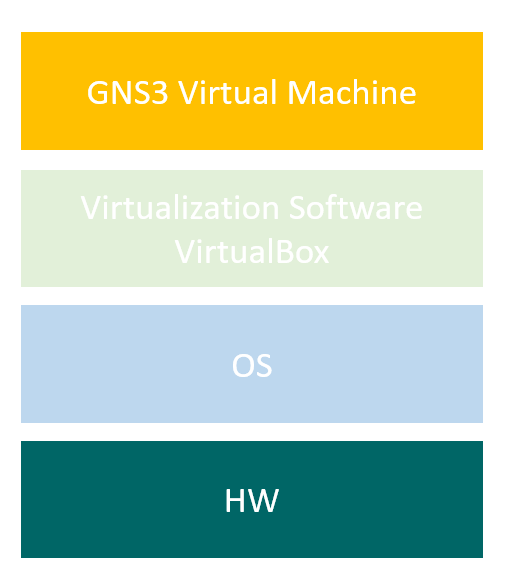
\includegraphics[width=0.5\textwidth]{graphics/Architecture_virtualbox.PNG}
	\caption{\en{Virtualization} Γενική αρχιτεκτονική}
\end{figure}

Με τη χρήση του \en{VirtualBox}, δημιουργήθηκε ένα εικονικό περιβάλλον όπου το \en{GNS3} μπορούσε να τρέξει τις προσομοιώσεις δικτύου, χωρίς την ανάγκη φυσικού εξοπλισμού. Αυτό μας έδωσε τη δυνατότητα να δοκιμάσουμε την εφαρμογή μας και να επαληθεύσουμε τη λειτουργικότητά της σε ένα ελεγχόμενο περιβάλλον, εξασφαλίζοντας ρεαλιστικά σενάρια προσομοίωσης.
Οι παρακάτω εικόνες βοηθούν στην κατανόηση της γενικής και ειδικής αρχιτεκτονικής που χρησιμοποιήθηκε



\FloatBarrier

Το \en{VirtualBox} χρησιμοποιήθηκε συνεπώς προκειμένου να σηκώσουμε το \en{GNS3 VM}. Οι \en{developers} του \en{GNS3} συνιστoύν για τις περισσότερες περιπτώσεις την εγκατάσταση και του \en{GNS3 VM} όταν χρησιμοποιoύμε \en{Windows OS}[27]. Συνεπώς το \en{GNS3 VM} ήταν σημαντικό να εγκατασταθεί καθώς αποτελούσε συστημικό στοιχείο του \en{GNS3} λογισμικού. Η αρχιτεκτονική της εικονοποίησης μπορεί να περιγραφεί με το σχήμα 4.2 με έναν πιο ειδικό τρόπο. Στο πρώτο επίπεδο βρίσκεται το υλικό, στο δεύτερο επίπεδο είναι το λειτουργικό σύστημα \en{windows}. Το επόμενο επίπεδο αποτελείται από το λογισμικό \en{VirtualBox}, το οποίο λειτουργεί ως \en{hypervisor} τύπου Β, παρέχοντας τη δυνατότητα δημιουργίας και διαχείρισης εικονικών μηχανών. Η εικονική μηχανή \en{GNS3 VM} εκτελείται εντός του \en{VirtualBox} και χρησιμεύει ως το περιβάλλον φιλοξενίας των εικόνων του λειτουργικού συστήματος \en{Cisco IOS}, οι οποίες εκτελούνται πάνω σε αυτήν, επιτρέποντας την προσομοίωση και διαχείριση δικτυακών τοπολογιών με αποδοτικό και κλιμακούμενο τρόπο.



\begin{figure}[htb]
	\centering
	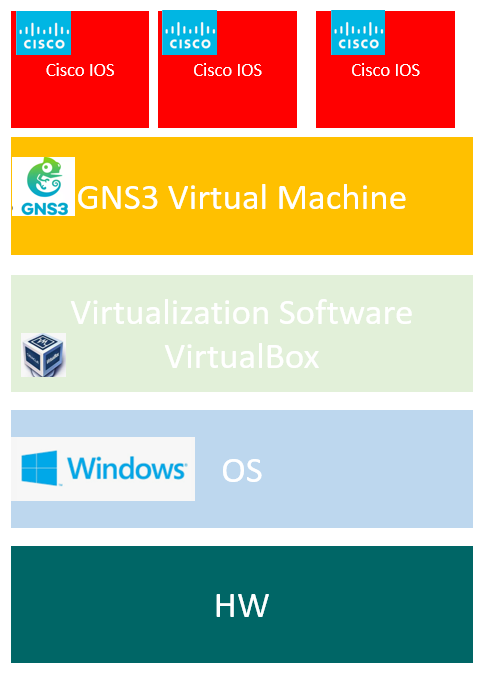
\includegraphics[width=0.5\textwidth]{graphics/virtualization_architecture.PNG}
	\caption{\en{Virtualization} Γενική αρχιτεκτονική}
\end{figure}

Στην εικόνα 4.3 μπορούμε να δούμε το περιβάλλον του \en{VirtualBox} και την εικονική μηχανή \en{GNS3 VM}.

\begin{figure}[htb]
	\centering
	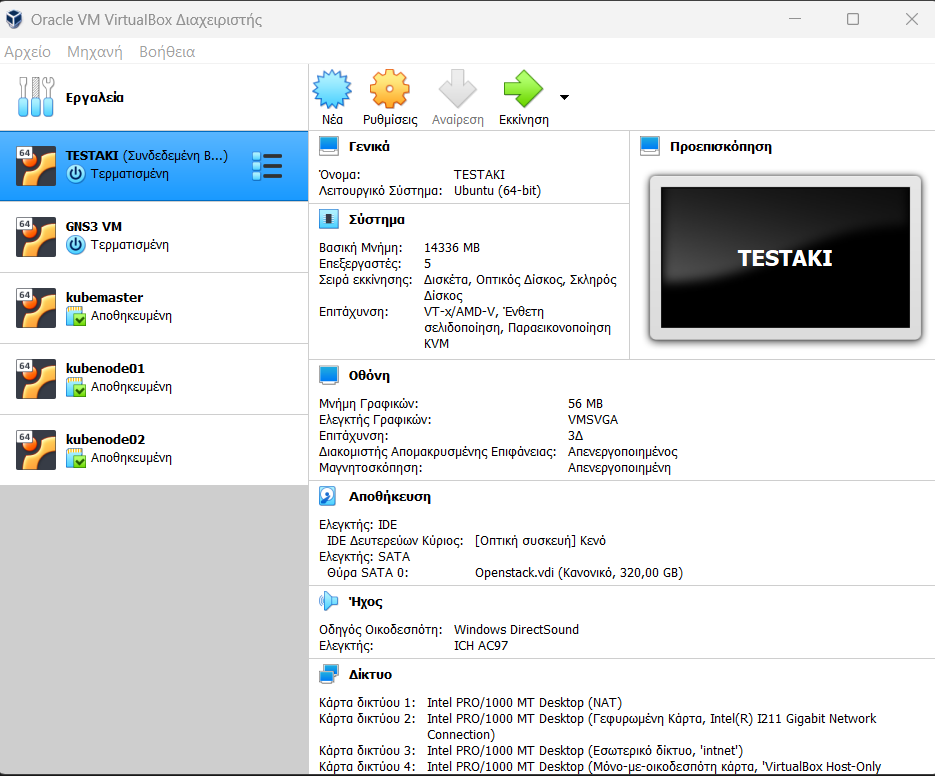
\includegraphics[width=0.9\textwidth]{graphics/virtualbox.PNG}
	\caption{\en{Virtualbox} }
\end{figure}


%\begin{equation}
%	y = \alpha x + \beta
%\end{equation}

%Αντίθετα με αυτό που θεωρεί η πλειοψηφία, το \en{Lorem Ipsum} δεν είναι απλά ένα τυχαίο κείμενο. Οι ρίζες του βρίσκονται σε ένα κείμενο Λατινικής λογοτεχνίας του 45 π.Χ., φτάνοντας την ηλικία του πάνω από 2000 έτη.


%\begin{figure}[htb]
%	\centering
%	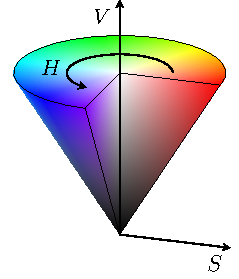
\includegraphics{tikz/hsv_cone/hsv_cone.pdf}
%	\caption{Ο χρωματικός χώρος \en{HSV}.}
%\end{figure}
